\markdownRendererHeadingFour{Arquitectura}\markdownRendererInterblockSeparator
{}\begin{figure}[h!] \centering 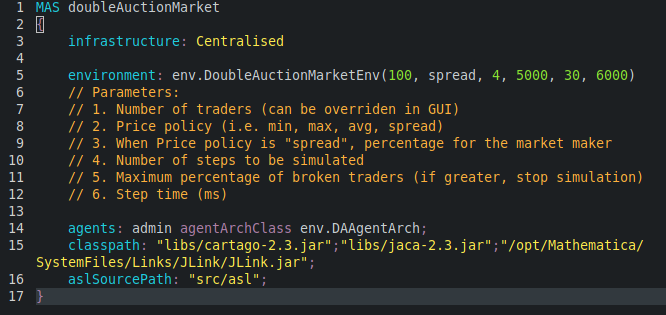
\includegraphics[scale=0.4]{img/code.png} \end{figure}\markdownRendererInterblockSeparator
{}\markdownRendererUlBegin
\markdownRendererUlItem This is the template I created for my poster presentations. \markdownRendererCite{1}+{}{}{novotny:2017}\markdownRendererUlItemEnd 
\markdownRendererUlItem You can provide an optional \texttt{\textbackslash footimage}. \markdownRendererCite{1}+{}{}{novotny:2019}\markdownRendererUlItemEnd 
\markdownRendererUlEnd \markdownRendererInterblockSeparator
{}\markdownRendererHorizontalRule{}\markdownRendererInterblockSeparator
{}\markdownRendererHeadingFour{Options}\markdownRendererInterblockSeparator
{}\markdownRendererUlBegin
\markdownRendererUlItem It's based on \texttt{beamerposter}, so you can change some options:\markdownRendererInterblockSeparator
{}\markdownRendererDlBegin
\markdownRendererDlItem{size}\markdownRendererDlDefinitionBegin a0, a0b, a1, a2, a3, a4\markdownRendererDlDefinitionEnd \markdownRendererDlItemEnd \markdownRendererDlItem{orientiation}\markdownRendererDlDefinitionBegin landscape, portrait\markdownRendererDlDefinitionEnd \markdownRendererDlItemEnd \markdownRendererDlItem{scale}\markdownRendererDlDefinitionBegin a decimal number to scale the fonts\markdownRendererDlDefinitionEnd \markdownRendererDlItemEnd 
\markdownRendererDlEnd\markdownRendererUlItemEnd 
\markdownRendererUlEnd \markdownRendererInterblockSeparator
{}\markdownRendererHorizontalRule{}\markdownRendererInterblockSeparator
{}\markdownRendererHeadingFour{Simulación de precios}\markdownRendererInterblockSeparator
{}Al evaluar los resultados añadiendo mayor proporción de agentes que siguen la estrategia Moving Average (MA) se observa que el comportamiento de la serie de tiempo de precios adquiere periodicidad hasta llegar a un punto crítico entre 75\% y 80\% de agentes MA en donde la simulación converge a un precio estacionario.\markdownRendererInterblockSeparator
{}\begin{figure}[h!] \centering 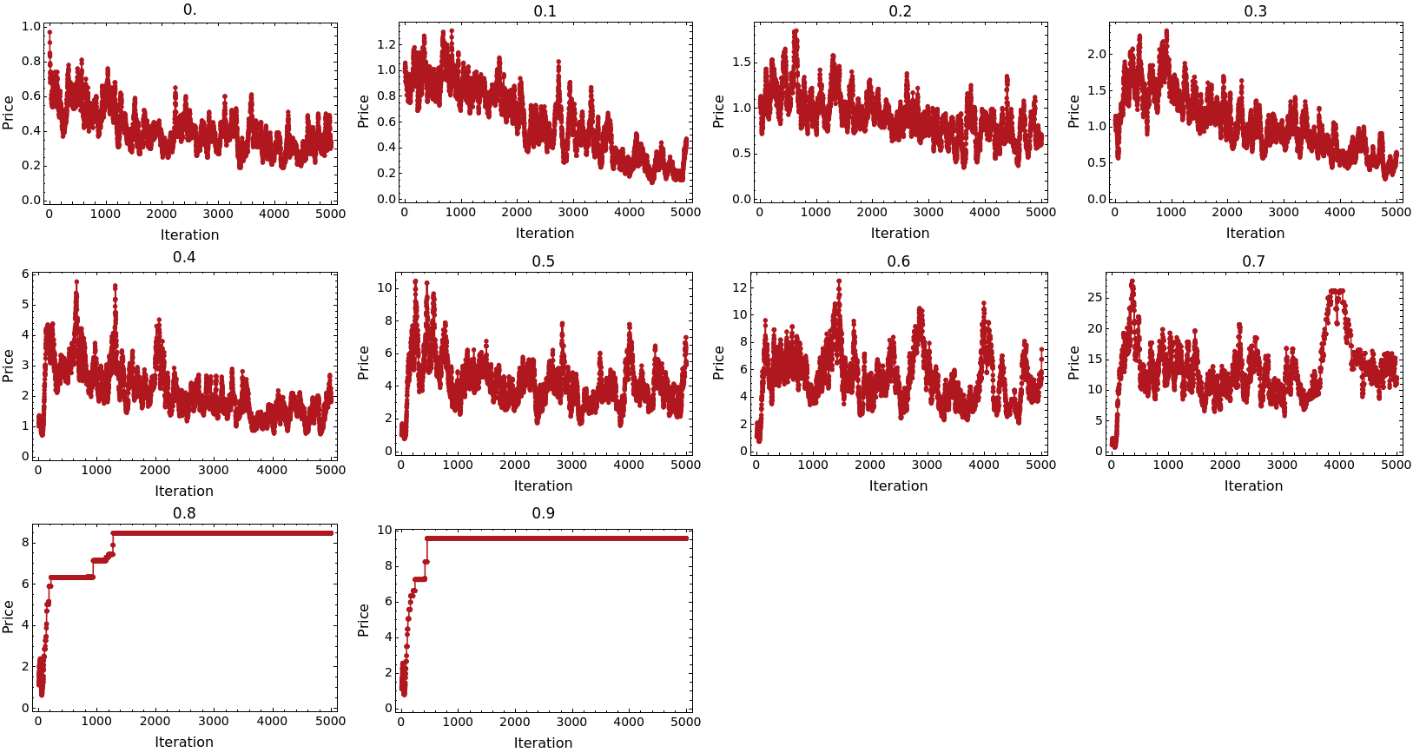
\includegraphics[scale=0.2]{img/price_series.png} \end{figure}\markdownRendererInterblockSeparator
{}\markdownRendererHorizontalRule{}\relax